
%%%%%%%%%%%%%%%%%%%%%
\section{Pendule simple}
%%%%%%%%%%%%%%%%%%%%%
%
%\subsection{Définition}

%Un champ est la donnée de sa valeur en tout point de l'espace. Cette valeur peut être scalaire ou vectoriel. Elle peut éventuellement être variable au cours du temps, elle est généralement variable dans l'espace.

\subsection{Définition}

Un pendule simple est une masse suspendue à une tige rigide pouvant pivoter en un point. Un tel dispositif possède une position d'équilibre, et un mouvement oscillatoir autour de cette position.



%%%%%%%%%%%%%%%%%%%%%
\section{Oscillateur harmonique}
%%%%%%%%%%%%%%%%%%%%%

\begin{center}
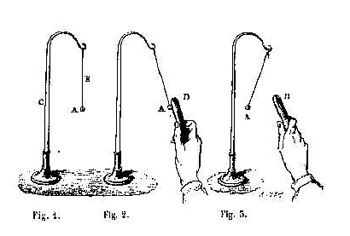
\includegraphics[scale=0.9]{./theorieDesChamps/MascartTraiteDElectriciteStatique1876}
\end{center}

\begin{minipage}[c]{.45\linewidth}
\begin{center}
Vision "Force de Coulomb"
\end{center}
Une charge électrique $Q_1$ exerce une force de Coulomb $\overrightarrow{F}_{Q_1/Q_2}$ sur la charge électrique $Q_2$
\setlength{\unitlength}{1cm}
\begin{picture}(10,3)
\put(0.5,1.0){\circle{0.3}}
\put(0.3,0.3){$Q_1$}
%\put(0.5,1.0){\vector(1,0){1.36}}
%\put(1.2,1.3){$\overrightarrow{F}_{Q_2/Q_1}$}
\put(5.5,1.0){\circle{0.5}}
\put(5.3,0.2){$Q_2$}
\put(5.5,1.0){\vector(-1,0){1.36}}
\put(3.7,1.3){$\overrightarrow{F}_{Q_1/Q_2}$}
\end{picture}
%On peut alors se demander comment l'information de la présence de $Q_1$ parvient à $Q_2$, y a-t-il quelque chose qui se propage entre les charges ? Cette question peut être simplifiée en disant que les charges créent un champ dans tout l'espace et qu'elle sont sensibles à ce champ.
\end{minipage}
\hfill
\begin{minipage}[c]{.45\linewidth}
\begin{center}
Vision "Champ électrique"
\end{center}
Une charge électrique $Q_1$ crée un champ électrique $\overrightarrow{E}$ dans tout l'espace.
\setlength{\unitlength}{1cm}
\begin{picture}(10,3)
\put(0.5,1.0){\circle{0.3}}
\put(0.3,0.3){$Q_1$}
\put(5.5,1.0){\vector(-1,0){1.36}}
\put(3.7,1.3){$\overrightarrow{E}$}
\end{picture}
Le champ électrique $\overrightarrow{E}$ exerce une force $\overrightarrow{F}_{\overrightarrow{E}/Q_2}$ sur la charge électrique $Q_2$
\setlength{\unitlength}{1cm}
\begin{picture}(10,3)
\put(5.5,1.0){\circle{0.5}}
\put(5.3,0.2){$Q_2$}
\put(5.5,1.0){\vector(-1,0){1.36}}
\put(3.7,1.3){$\overrightarrow{F}_{\overrightarrow{E}/Q_2}$}
\end{picture}
\end{minipage}

Le champ créé par une charge électrique est à priori un outil purement mathématique, un artifice de calcul bien pratique. L'existence de ce "champ électrique" est à priori hypothétique. Néanmoins, son existence permet d'interpréter la transmission de "l'information de présence" entre les charges, de lever l'hypothèse d'une transmission d'information instantanée et immatérielle entre les charges.

\subsection{Champ magnétique}

De la même façon que pour l'électrostatique, les physiciens vont introduire le champs magnétique afin de "nommer à priori" le "médiateur" entre les aimants "expliquant" leurs interactions.

\subsection{Autres exemples de champs}

Champ de température dans l'atmosphère terrestre, champ d'altitude sur une carte topographique.

%%%%%%%%%%%%%%%%%%%%%%%%%%%%%%%%%%%%%%%%%%%%%%%%%%%%%%%%%%%%%%%%%%%%%%%%%%%%
